\subsection{UC12 - Cancellazione scaffalatura}
\begin{figure}[H]
  \centering
  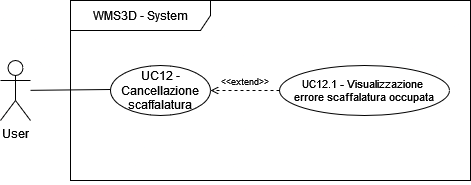
\includegraphics[width=0.8\textwidth]{UC_diagrams_11-20/UC12_sys.drawio.png}
   \caption{Diagramma UML UC12 - Cancellazione scaffalatura}
\end{figure}
\begin{figure}[H]
  \centering
  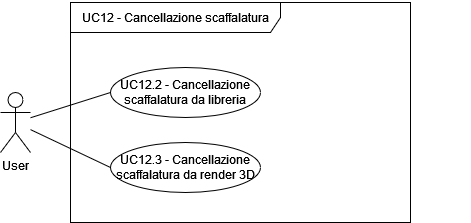
\includegraphics[width=0.8\textwidth]{UC_diagrams_11-20/UC12.drawio.png}
   \caption{Diagramma UML in dettaglio UC12 - Cancellazione scaffalatura}
\end{figure}
\begin{itemize}
    \item \textbf{Attori:} User.
    \item \textbf{Pre-condizione:} L'utente ha selezionato una scaffalatura [UC8].
    \item \textbf{Post-condizione:} La scaffalatura viene eliminata.
    \item \textbf{Scenario Principale:} L'utente elimina da libreria [UC12.2] e dal render 3D [UC12.3] la scaffalatura precedentemente selezionata.
    \item \textbf{Generalizzazioni:} -
    \item \textbf{Estensioni:} È presente una estensione:
    \begin{itemize}
        \item UC12.1 - Visualizzazione errore scaffalatura occupata.
    \end{itemize}
\end{itemize}


\subsubsection{UC12.1 - Visualizzazione errore scaffalatura occupata}
\begin{itemize}
    \item \textbf{Attori:} User.
    \item \textbf{Pre-condizione:} L'utente vuole cancellare una scaffalatura [UC12] con prodotti posizionati all'interno.
    \item \textbf{Post-condizione:} L'utente visualizza un messaggio d'errore e l'operazione fallisce.
    \item \textbf{Scenario Principale:} L'utente visualizza un messaggio informativo sull'errore e ne conferma la ricezione. L'operazione fallisce e l'utente se vuole eliminare quella scaffalatura dovrà spostarne i prodotti.   
    \item \textbf{Generalizzazioni:} -
    \item \textbf{Estensioni:} -
\end{itemize}


\subsubsection{UC12.2 - Cancellazione scaffalatura da libreria}
\begin{itemize}
    \item \textbf{Attori:} User.
    \item \textbf{Pre-condizione:} L'utente ha selezionato una scaffalatura [UC8] e la vuole eliminare.
    \item \textbf{Post-condizione:} L'utente elimina la scaffalatura dalla libreria.
    \item \textbf{Scenario Principale:} L'utente elimina da libreria la scaffalatura precedentemente selezionata.   
    \item \textbf{Generalizzazioni:} -
    \item \textbf{Estensioni:} -
\end{itemize}


\subsubsection{UC12.3 - Cancellazione scaffalatura da render 3D}
\begin{itemize}
    \item \textbf{Attori:} User.
    \item \textbf{Pre-condizione:} L'utente ha selezionato una scaffalatura [UC8] e la vuole eliminare.
    \item \textbf{Post-condizione:} L'utente elimina la scaffalatura dal render 3D.
    \item \textbf{Scenario Principale:} L'utente elimina dal render 3D la scaffalatura precedentemente selezionata.   
    \item \textbf{Generalizzazioni:} -
    \item \textbf{Estensioni:} -
\end{itemize}